\documentclass[border=4pt]{standalone}
% Shared typography and colours for the standalone figures.
\usepackage{unicode-math}
\setmainfont{TeX Gyre Termes}
\setmathfont{TeX Gyre Termes Math}
\usepackage{tikz}
\usetikzlibrary{arrows.meta,positioning,calc,decorations.pathreplacing}
\usepackage{pgfplots}
\pgfplotsset{compat=1.18}

% One colour per element or subsystem. Record the mapping in
% the working repository conventions and use it identically in every figure.
\definecolor{elemA}{HTML}{1F5FA8}
\definecolor{elemB}{HTML}{B8461B}
\definecolor{elemC}{HTML}{2E7D32}
\definecolor{elemD}{HTML}{6A4C93}
\definecolor{frameline}{HTML}{555555}

% Article-specific diagram styling; common figure-style.tex remains managed.
\usepackage{circuitikz}
\usetikzlibrary{decorations.pathmorphing,fit,backgrounds}
\tikzset{
  every node/.style={font=\small},
  block/.style={draw=frameline,rounded corners=2pt,minimum height=7mm,align=center,fill=white},
  massA/.style={draw=elemA,fill=elemA!10,thick},
  massB/.style={draw=elemB,fill=elemB!10,thick},
  receiver/.style={draw=elemC,fill=elemC!9,thick},
  mediator/.style={draw=elemD,fill=elemD!8,thick},
  flow/.style={-{Latex[length=2.3mm]},thick},
  boundary/.style={draw=frameline,dashed,rounded corners=3pt},
  spring/.style={decorate,decoration={coil,aspect=.4,segment length=3mm,amplitude=1.5mm},thick,elemD}
}

\begin{document}
\begin{tikzpicture}
\path[use as bounding box] (0,-.5) rectangle (15,3.45);
\node[font=\small\bfseries] at (3.55,3.15) {Before contact};
\node[font=\small\bfseries] at (11.35,3.15) {After elastic release};
\draw[frameline!45] (7.3,-.2)--(7.3,3.3);
\draw[massA] (1.0,1.05) rectangle (2.0,1.8);
\draw[massB] (4.35,1.05) rectangle (6.15,1.8);
\node at (1.5,1.42) {$m$};
\node at (5.25,1.42) {$3m$};
\draw[flow,elemA] (1.5,2.12)--(3.6,2.12);
\node[above] at (2.5,2.12) {$p_1=p_0$};
\node[above] at (5.25,2.12) {$p_2=0$};
\node[align=center] at (3.55,.26) {$P=p_0$\qquad $A_p=p_0$\\$K=\tfrac12mu^2$};
\draw[massA] (8.6,1.05) rectangle (9.6,1.8);
\draw[massB] (11.5,1.05) rectangle (13.3,1.8);
\node at (9.1,1.42) {$m$};
\node at (12.4,1.42) {$3m$};
\draw[flow,elemA] (9.3,2.12)--(8.25,2.12);
\draw[flow,elemB] (10.75,2.12)--(13.9,2.12);
\node[above] at (8.75,2.12) {$-\tfrac12p_0$};
\node[above] at (12.4,2.12) {$+\tfrac32p_0$};
\node[align=center] at (11.35,.26) {$P=p_0$\qquad $A_p=2p_0$\\$K=\tfrac12mu^2$};
\end{tikzpicture}
\end{document}
